\documentclass[12pt,a4paper]{article}
\usepackage[utf8x]{inputenc}
\usepackage{ucs}
\usepackage[english,russian]{babel}
\usepackage[OT1]{fontenc}
\usepackage{amsmath}
\usepackage{amsfonts}
\usepackage{amssymb}
\usepackage{wasysym}
\usepackage{physics}
\usepackage{wrapfig}
\usepackage{mathrsfs}

%---------Схемы---------
\usepackage{circuitikz}
%-----------------------

%--------Графики--------
\usepackage{pgfplots}
%Чтобы хорошо работало
\pgfplotsset{compat=1.9}
%----------------------

\usepackage[left=2cm,right=2cm,top=2cm,bottom=2cm,includefoot,footskip=1.5cm]{geometry}

\usepackage{fancyhdr}
\pagestyle{fancy}

\usepackage[T1]{fontenc}
 
\usepackage{indentfirst}
%% Sets page size and margins
%\usepackage[dvips]{graphicx}
%\graphicspath{{noiseimages/}}
%\usepackage[colorinlistoftodos]{todonotes}
%\usepackage[colorlinks=true, allcolors=blue]{hyperref}

\rhead{\small Д.\,Павлов, МФТИ}
\lhead{Лабораторная работа №3.3.5}

\author{Дмитрий Павлов, 790}
\title {\textbf{Эффект Холла в металлах.}}

\begin{document}
\maketitle
\newpage
\tableofcontents 

\newpage

\section{Вступление.}
    \subsection{Цель работы.}
        Исследовать зависимость ЭДС Холла от величины магнитного поля при различных токах через образец для определения константы Холла; определить знак носителей заряда и проводимость различных металлических образцов (медь, цинк, серебро).
        
    \subsection{Оборудование.}
        \begin{itemize}
            \item Электромагнит с источником питания;
            \item Источник постоянного тока;
            \item Микровольтметр Ф116/1;
            \item Амперметры;
            \item Измеритель магнитной индукции Ш1-10;
            \item Образцы из меди, серебра и цинка.
        \end{itemize}

    \subsection{Экспериментальная установка.}
        \begin{wrapfigure}{2}{0.6\linewidth}
        	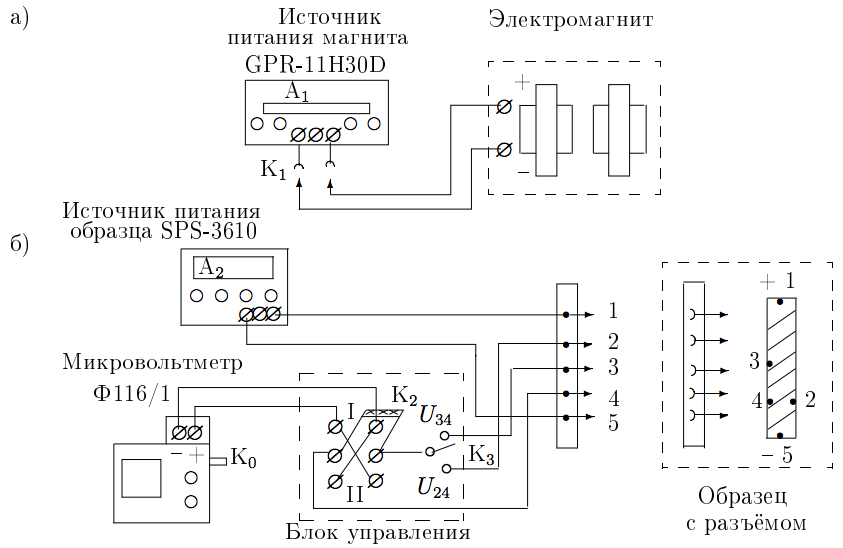
\includegraphics[width=\linewidth]{img/img1.png}
        	\hspace{44pt}{Рисунок 1 -- Схема установки для исследования эффекта Холла в металлах.}
        \end{wrapfigure}
        
        В зазоре электромагнита (рис. 1а) создается постоянное магнитное поле, величину которого можно менять с помощью регуляторов тока источника питания. Ток питания электромагнита измеряется амперметром источника $A_1$. Разъем $K_1$ позволяет менять направление тока в обмотках электромагнита.
        
        Градуировка магнита проводится с помощью измерителя магнитной индукции.
        
        Металлические образцы в форме тонких пластинок, смонтированные в специальных держателях, подключаются к блоку питания через разъем (рис. 1б). Ток через образец регулируется ручками источника и измеряется амперметром источника $A_2$.
        
        В образце с током, помещенном в зазор электромагнита, между контактами 2 и 4 возникает холловская разность потенциалов, которая измеряется с помощью микровольтметра Ф116/1, если переключатель $K_3$ подключён к точке 2 образца. При подключении $K_3$ в точке $3$ микровольтметр измеряет омическое падение напряжения $U_{34}$, вызванное основным током через образец. При нейтральном положении ключа входная цепь микровольтметра разомкнута.

        Ключ $K_2$ позволяет менять полярность напряжения, поступающего на вход микровольтметра.
        
        Измеряемая разность потенциалов при одном направлении магнитного поля равна сумме ЭДС Холла и омического падения напряжения, а при другом - их разности.
        
        По знаку $\varepsilon_x$ можно определить характер проводимости --- электронный или дырочный. Для этого необходимо знать направление тока в образце и направление магнитного поля.
        
        Измерив ток $I$ в образце и напряжение $U_{34}$ между контактами $3$ и $4$ в отсутствие магнитного поля, можно, зная параметры образца, рассчитать проводимость материала образца по формуле:
        \[
        \sigma = I \cdot L_{34}/(U_{34}\cdot a \cdot l),
        \]
        где $L_{34}$ - расстояние между контактами $3$ и $4$, $a$ - толщина образца, $l$ - его ширина.
        
\newpage
\section{Измерения.}
    \subsection{Градуировка электромагнита.}
        С помощью измерителя магнитной индукции Ш1-10 исследуем зависимость индукции $B$ магнитного поля в зазоре электромагнита от тока через магнит.
        
        Проведем измерения магнитной индукции $B$ для $6-8$ значений тока через электромагнит $I_M$ (вплоть до максимального $I_M$). Результаты проведенных измерений находятся в таблице 1.
        
        \begin{table}[!h]
            \begin{flushleft}%\hspace{80}
           		\textbf{Таблица 1} -- Зависимость индукции $B$ магнитного поля в зазоре электромагнита от тока через магнит.\\
            \end{flushleft}
            \begin{center}
                \begin{tabular}{ | l | l | l | l | l | l | l | l | l | l |}
                    \hline
                    $I$, мА &   0.15    &   0.25    &   0.4     &   0.55    &   0.7     &   0.85    &   1       &   1.15    &   1.28    \\
                    \hline
                    $B$, мТл&   174.3   &   304.7   &   488.4   &   665     &   812.2   &   935.4   &   1011.4  &   1065.3  &   1103.8  \\
                    \hline                
                \end{tabular}
            \end{center}
        \end{table}
    
        На рисунке 2 изображена зависимость индукции $B$ магнитного поля в зазоре электромагнита от тока (данные из таблицы 1). 
        
    \subsection{Измерение ЭДС Холла.}
        \subsubsection{Зависимость ЭДС Холла от тока в электромагните для семи фиксированных    значений тока для медной пластинки.}
            Снимем зависимость напряжения $U_{24}$ (включая $U_0$) от тока $I_M$ через обмотки магнита при фиксированном токе через образец. Сделаем семь серий измерений, первую  при токе $I_\text{обр} = 0.2A$, последнюю при $I_\text{обр} = 0.97A$ (максимальный ток). Результаты измерений находятся в таблице 2. 
        
            По данным из таблицы 2 построим семейство графиков зависимостей напряжения $U_{24}$ от тока $I_\text{м}$ через обмотки магнита при различных фиксированных токах через образец --- рисунок 3.
        
        \subsubsection{Зависимость ЭДС Холла от тока в электромагните для цинковой пластинки.}
            Для образца из цинка снимем зависимость $U = f(I_\text{м})$ при одном значении тока через образец. Результаты измерений находятся в таблице 3. 
        
            По данным из таблицы 3 построим график --- зависимость ЭДС Холла от тока для цинковой пластины --- рисунок 4.
            
    \subsection{Определение характера проводимости.}
        У материалов с преобладающей электронной проводимостью постоянная Холла отрицательна, с дырочной проводимостью - положительная. 
        
        Получаем что основные носители заряда у меди - электроны, у цинка - дырки.

    \subsection{Определение удельной проводимости.}
        При токе через образец $I \simeq 1$ А падение напряжения между контактами $3$ и $4$ для каждого из образцов оказалось равным: $U(Zn) = 312$ мкВ, $U(Cu) = 280$ мкВ.
        
        Медная пластинка:
        \begin{itemize}
            \item $L = 7.5$ мм.
            \item $l = 8$ мм.
            \item $a = 0.05$ мм.
        \end{itemize}
        
        Цинковая пластинка:
        \begin{itemize}
            \item $L = 4$ мм.
            \item $l = 10$ мм.
            \item $a = 0.08$ мм.
        \end{itemize}
\newpage        
\section{Обработка результатов.}
    \subsection{Градуировка электромагнита.}
        В пункте 3.1 построили график зависимости индукции магнитного поля от тока через электромагнит: $B = f(I_\text{М})$ --- рисунок 2.
        
        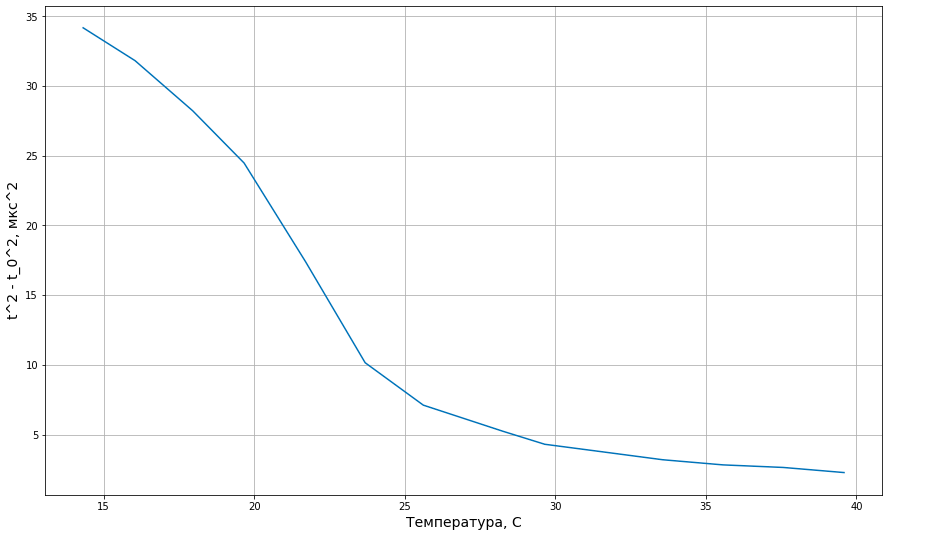
\includegraphics[width=0.8\linewidth]{img/img2.png}
	
	    \textbf{Рисунок 2} -- Зависимость индукции $B$ магнитного поля в зазоре электромагнита от тока через магнит.
        
    \subsection{Семейство характеристик $\mathcal{E}_x = f(B)$ при различных значениях тока $I$ через образец для меди.}
        В пункте 3.2.1 нашли ЭДС Холла и построили семейство характеристик $\mathcal{E}_x = f(B)$ при различных значениях тока $I$ через образец для меди --- рисунок 3. Определим угловые коэффициенты $K(I) = \Delta \mathcal{E}_x/\Delta B$ полученных прямых. Результаты находятся в таблице 4.
        
        \begin{table}[!h]
            \begin{flushleft}%\hspace{80}
           		\textbf{Таблица 4} -- Угловые коэффициенты полученных прямых. Уравнения в виде $y = bx + a$, два правых столбика - погрешности $b$ и $a$ соответственно.\\
            \end{flushleft}
            \begin{center}
                \begin{tabular}{ | l | l | l | l |}
                    \hline
                    $b$      &   $a$    &   $\sigma_b$&   $\sigma_a$\\
                    \hline
                    0.022   &   -1.412  &   0.001   &   0.464   \\
                    \hline      
                    0.033   &   -1.967  &   0.002   &   0.628   \\
                    \hline    
                    0.045   &   -2.272  &   0.002   &   0.853   \\
                    \hline 
                    0.057   &   -2.053  &   0.003   &   1.081   \\
                    \hline 
                    0.071   &   -3.106  &   0.004   &   1.242   \\
                    \hline 
                    0.082   &   -1.678  &   0.005   &   1.553   \\
                    \hline 
                    0.094   &   -1.968  &   0.005   &   1.711   \\
                    \hline    
                \end{tabular}
            \end{center}
        \end{table}
    
        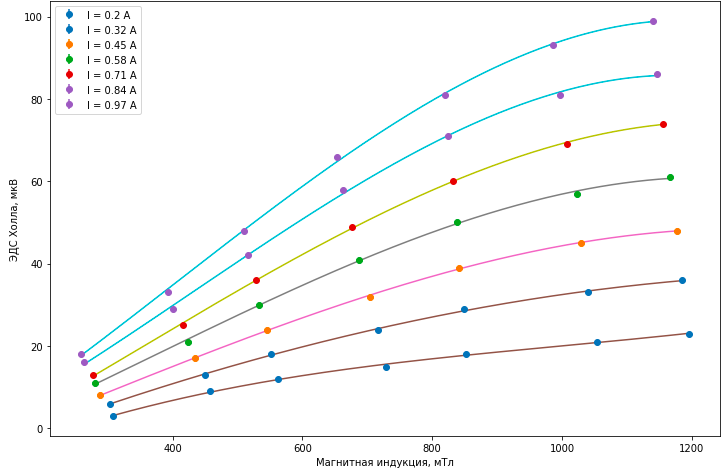
\includegraphics[width=0.9\linewidth]{img/img3.png}
	
	    \textbf{Рисунок 3} -- Зависимость напряжения $U_{24}$ от тока $I_M$ через обмотки магнита при фиксированном токе через образец.

		
	\subsection{$\mathcal{E}_x = f(B)$ при максимальном токе $I$ через образец из цинка.}
		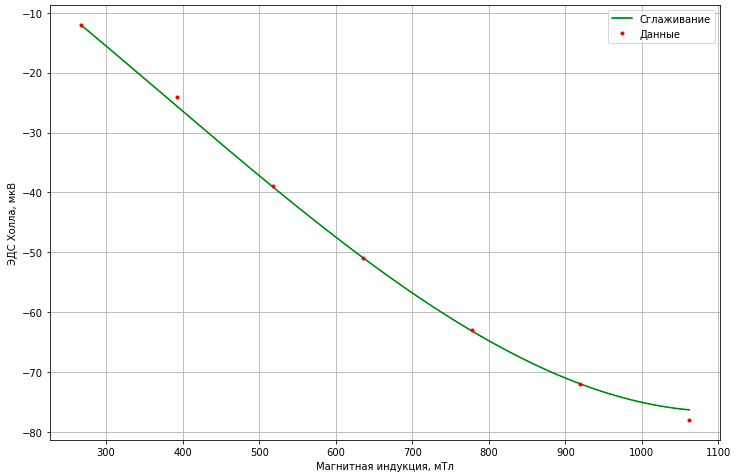
\includegraphics[width=0.9\linewidth]{img/img4.png}
		
        \textbf{Рисунок 4} -- Зависимость ЭДС Холла от индукции при различных значениях тока через цинковый образец.
        
        \begin{table}[!h]
            \begin{flushleft}%\hspace{80}
           		\textbf{Таблица 7} -- Прямая ЭДС Холла для цинка. Уравнение в виде $y = bx + a$, два правых столбика - погрешности $b$ и $a$ соответственно.\\
            \end{flushleft}
            \begin{center}
                \begin{tabular}{ | l | l | l | l |}
                    \hline
                    $b$     &   $a$    &   $\sigma_b$ &   $\sigma_a$\\
                    \hline
                    0.095   &   -1.968 &    0.006   &   1.711   \\
                    \hline    
                \end{tabular}
            \end{center}
        \end{table}
        
    \subsection{Коэффициента наклона $\dfrac{\Delta \mathcal{E}_\text{Холла}}{\Delta B}$ от тока $I$ через образец.}
        Из серии измерений ЭДС Холла при различных фиксированных токах через образец в зависимости от магнитной индукции, создаваемой электромагнитом, построим график зависимости углового коэффициента наклона $\dfrac{\Delta \mathcal{E}_\text{Холла}}{\Delta B}$ от тока $I$ через образец.
        \begin{table}[!h]
            \begin{flushleft}%\hspace{80}
           		\textbf{Таблица 5} -- Зависимость угла наклона $\Delta \mathcal{E}_\text{Холла}/\Delta B$ от тока через образец.\\
            \end{flushleft}
            \begin{center}
                \begin{tabular}{ | l | l | l | l | l | l | l | l |}
                    \hline
                    $I_\text{обр}$, A& 0.2   & 0.32  & 0.45  & 0.58  & 0.71  & 0.84  & 0.97   \\
                    \hline      
                    $K$         & 0.094 & 0.082 & 0.071 & 0.057 & 0.045 & 0.034 & 0.022   \\
                    \hline    
                \end{tabular}
            \end{center}
        \end{table}
        
        По данным таблиц 4 и 5 построим требуемый график --- рисунок 5. 
        \begin{center}
            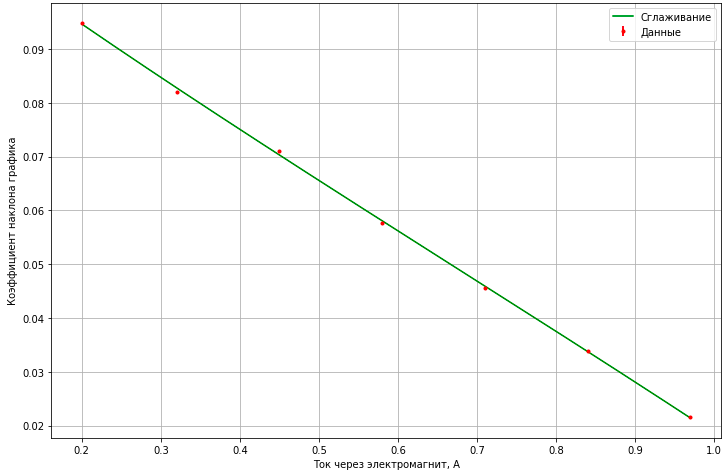
\includegraphics[width=0.72\linewidth]{img/img5.png}
	
	        \textbf{Рисунок 5} -- Зависимость угла наклона $\Delta \mathcal{E}_\text{Холла}/\Delta B$ от тока через образец. 
        \end{center}

        При этом параметры полученной прямой $y = bx + a$: 
        \[
        b = -0.095; a = 0.113; 
        \]
        \[
        \sigma(b) =  0.001; \sigma(a) =  0.001.
        \]
	    
    \subsection{Постоянная Холла для меди, $R_\text{Х}$.}
        ЭДС Холла выражается так:
        \[
        \mathcal{E}_x = -R_\text{x}\cdot \dfrac{IB}{a},
        \]
        где $a$ - толщина пластинки; $R_\text{х}$ - постоянная Холла.
        
        Отсюда выразим постоянную Холла $R_\text{х}$:
        \[
        R_\text{х} = - \dfrac{a\mathcal{E_\text{х}}}{IB}.
        \]
        
        Результаты находятся в таблице 6.
        \begin{table}[!h]
            \begin{flushleft}%\hspace{80}
           		\textbf{Таблица 6} -- Постоянная Холла для медного образца.\\
            \end{flushleft}
            \begin{center}
                \begin{tabular}{ | l | l | l | l | l | l | l | l |}
                    \hline
                    $I_\text{обр}$, A                & 0.2   & 0.32  & 0.45  & 0.58  & 0.71  & 0.84  & 0.97   \\
                    \hline      
                    $R_\text{Х} \cdot 10^{-9}$  & 0.23  & 0.13  & 7.8   & 4.9   & 3.2   & 2.0   & 1.1   \\
                    \hline    
                    $sigma_{R_X} \cdot 10^{-9}$  & 0.02  & 0.01  & 0.6   & 0.5   & 0.3  & 0.2   & 0.1   \\
                    \hline    
                \end{tabular}
            \end{center}
        \end{table}
        
        \[
        <R_X> = -7.658 \cdot 10^{-9}.
        \]
        \[
        sigma_{R_X} = 0.8 \cdot 10^{-9}.
        \]
        \[
        \varepsilon_{R_X} = 0.1 = 10\%.
        \]
    \subsection{Постоянная Холла для цинка, $R_\text{Х}$.}
        Аналогично 4.4 находим постоянную Холла для цинка: $R_\text{х} = - \dfrac{a\mathcal{E_\text{х}}}{IB} = +7.6\cdot 10^{-9}$. $ \varepsilon_{R_X} = 0.1 = 10\%.$ Положительный знак этой величины свидетельствует о дырочной проводимости образца. 
        
    \subsection{Концентрация $n$ носителей тока.}
    Почти по определению постоянная Холла:
    \[
    R_\text{х} = \dfrac{1}{ne},
    \]
    откуда получаем выражение для оценки концентрации носителей тока в проводнике: $n = \dfrac{1}{R_\text{х}e}.$
    Тогда носителей заряда в меди в зависимости от тока $I$ --- смотри таблицу 8.
    Результат для цинка: $n = \dfrac{1}{R_\text{х}e} = 1.37\cdot 10^{27}$ единиц.
    
    \begin{table}[!h]
        \begin{flushleft}%\hspace{80}
       		\textbf{Таблица 8} -- Носителей заряда в меди.\\
        \end{flushleft}
        \begin{center}
            \begin{tabular}{ | l | l | l | l | l | l | l | l |}
                \hline
                $I_\text{обр}$, А   &   0.2     & 0.32  & 0.45  &   0.58    &   0.71    &   0.84    &   0.97  \\
                \hline
                $n$, $10^{27}$ ед   &   0.263   & 0.487 & 0.790 &   1.25    &   1.94    &   3.09    &   5.63  \\
                \hline    
                $\sigma_n$, $10^{26}$ ед   &   0.1   & 0.35 & 0.6 &   1.1    &   1.8    &   2.7    &   5 \\
                \hline    
            \end{tabular}
        \end{center}
    \end{table}
    \[
    \varepsilon_n = 0.7 = 7\%.
    \]
    
    Среднее значение: $n_\text{ср} = 1.92 \cdot 10^{27}$ ед.
    \subsection{Удельная проводимость $\sigma$ образцов.}
    Удельная проводимость образцов находится по формуле:
    \[
    \sigma = \dfrac{I \cdot L_{34}}{U_{34}\cdot a \cdot l},
    \]
    где $L_{34}$ - расстояние между контактами 3 и 4, $a$ - толщина пластинки, $l$ - ширина пластинки.
    
    Значения $L_{34}$, $U_{34}$, $a$ и $l$ найдены в пункте 3.4. 
    
    Тогда удельная проводимость образцов:
    \[
    \sigma_\text{медь} = \dfrac{0.97 \text{ A} \cdot 7.5 \text{ мм}}{3.12 \text{ мВ}\cdot 0.05 \text{ мм} \cdot 8\text{ мм}} = 5.8 \cdot 10^{6} (\text{Ом}\cdot \text{м})^{-1}.
    \]
    \[
    \sigma_\text{цинк} = \dfrac{0.97 \text{ A} \cdot 4 \text{ мм}}{2.8 \text{ мВ}\cdot 0.08 \text{ мм} \cdot 10\text{ мм}} = 1.7 \cdot 10^{6} (\text{Ом}\cdot \text{м})^{-1}.
    \]
    При этом табличные значения проводимости:
    \begin{itemize}
        \item $\sigma_\text{медь} = 5.95 \cdot 10^{6} (\text{Ом}\cdot \text{м})^{-1}$
        \item $\sigma_\text{цинк} = 1.69 \cdot 10^{6} (\text{Ом}\cdot \text{м})^{-1}$
    \end{itemize}
    
    \subsection{Подвижность $b$ носителей тока.}
    Определим подвижность носителей тока:
    \[
    b_\text{медь} = \dfrac{\sigma_\text{медь}}{en_1} = \dfrac{5.8 \cdot 10^{6} (\text{Ом}\cdot \text{м})^{-1}}{1.6 \cdot 10^{-19} \cdot 1.92 \cdot 10^{27}} = 188 \dfrac{\text{см}^2}{B\cdot c}.
    \]
    \[
    b_\text{цинк} = \dfrac{\sigma_\text{цинк}}{en_2} =  \dfrac{1.7 \cdot 10^{6} (\text{Ом}\cdot \text{м})^{-1}}{1.6 \cdot 10^{-19} \cdot 1.37 \cdot 10^{27}} = 77 \dfrac{\text{см}^2}{B\cdot c}.
    \]

    Погрешность складывается из погрешности измерения $\sigma_\text{металл}$ и $n_1$.
    \subsection{Итоговая таблица.}
        \begin{table}[!h]
            \begin{flushleft}%\hspace{80}
           		\textbf{Таблица 0} -- Результаты.\\
            \end{flushleft}
            \begin{center}
                \begin{tabular}{| l | l | l | l |}
                    \hline
                    Металл  &   $R_X \pm \Delta R_X$    &   Табл.$R_X$    &   Знак. нос.    \\
                    \hline
                    Медь    &   $-7.9 \cdot 10^9$   &  $-5.3 \cdot 10^9$   & -   \\
                    \hline
                    Цинк    &   $+7.6 \cdot 10^9$   &  $10.4 \cdot 10^9$   & +   \\
                    \hline
                    Металл  &   $n \pm \Delta n (\text{м})^{-3}\cdot 10^{27}$  &   $\sigma \pm \Delta \sigma (\text{Ом}\cdot \text{м})^-1 \cdot 10^{6}$ &   $b, (\text{см})^2/(B\cdot c)$   \\
                    \hline
                    Медь    &   1.92    &   5.8    &   188     \\
                    \hline
                    Цинк    &   1.37    &   1.7    &   77   \\
                    \hline
                \end{tabular}
            \end{center}
        \end{table}

\newpage
\section{Таблицы.}

    \begin{table}[!h]
    \begin{flushleft}%\hspace{80}
   		\textbf{Таблица 2} -- Зависимость напряжения $U_{24}$ (включая $U_0$) от тока $I_M$ через обмотки магнита при фиксированном токе через образец.\\
    \end{flushleft}
        \begin{center}
            \begin{tabular}{ | l | l | l | l | l | l | l | l |}
                \hline
                $I_\text{обр} = 0.2$ A   &&&&&&& \\
                \hline
                $I$, мА     &   0.2     & 0.38  & 0.50  & 0.7   & 0.85  & 1.09      & 1.26      \\
                $B$, мТл    &   308.5   & 457.27& 561.73& 728.16& 851.73& 1053.64   & 1195.96   \\
                $E_x$, мкВ  &   3       & 9     & 12    & 15    & 18    & 21        & 23        \\
                \hline        
                $I_\text{обр} = 0.32$ A  &&&&&&& \\
                \hline
                $I$, мА     &   0.19    &   0.36& 0.49  & 0.68  & 0.84  & 1.08      & 1.24      \\
                $B$, мТл    &   303.21  & 450.11& 552.36& 716.60& 849.15& 1040.48   & 1184.19   \\
                $E_x$, мкВ  &   6       & 13    & 18    & 24    & 29    & 33        & 36        \\
                \hline     
                $I_\text{обр} = 0.45$ A  &&&&&&& \\
                \hline
                $I$, мА     &   0.18    & 0.35  & 0.48  & 0.67  & 0.84  & 1.07      & 1.22      \\
                $B$, мТл    &   287.84  & 434.95& 544.99& 704.04& 840.57& 1029.32   & 1177.43   \\
                $E_x$, мкВ  &   8       & 17    & 24    & 32    & 39    & 45        & 48        \\
                \hline   
                $I_\text{обр} = 0.58$ A  &&&&&&& \\
                \hline
                $I$, мА     &   0.16    & 0.34  & 0.47  & 0.65  & 0.83  & 1.06      & 1.21      \\
                $B$, мТл    &   280.47  & 423.79& 532.62& 686.49& 837.99& 1023.16   & 1166.66   \\
                $E_x$, мкВ  &   11      & 21    & 30    & 41    & 50    & 57        & 61        \\
                \hline   
                $I_\text{обр} = 0.71$ A  &&&&&&& \\
                \hline
                $I$, мА     &   0.16    & 0.33  & 0.46  & 0.64  & 0.83  & 1.04      & 1.2       \\
                $B$, мТл    &   278.09  & 415.62& 528.24& 675.93& 831.40& 1006.99   & 1154.89   \\
                $E_x$, мкВ  &   13      & 25    & 36    & 49    & 60    & 69        & 74        \\
                \hline   
                $I_\text{обр} = 0.84$ A  &&&&&&& \\
                \hline
                $I$, мА     &   0.15    & 0.32  & 0.45  & 0.62  & 0.82  & 1.03      & 1.2       \\
                $B$, мТл    &   263.72  & 401.46& 515.87& 662.37& 823.82& 996.83    & 1146.13   \\
                $E_x$, мкВ  &   13      & 16    & 29    & 42    & 58    & 71        & 81, 86    \\
                \hline   
                $I_\text{обр} = 0.97$ A  &&&&&&& \\
                \hline
                $I$, мА     &   0.14    & 0.30  & 0.44  & 0.61  & 0.81  & 1.01      & 1.19      \\
                $B$, мТл    &   258.35  & 392.30& 510.50& 653.81& 819.24& 986.67    & 1139.36   \\
                $E_x$, мкВ  &   18      & 33    & 48    & 66    & 81    & 93        & 99   \\
                \hline   
            \end{tabular}
        \end{center}
    \end{table}
    \begin{table}[!h]
        \begin{flushleft}%\hspace{80}
       		\textbf{Таблица 3} -- Зависимость $U = f(I_\text{м})$ для образца из цинка при одном значении тока $I_\text{обр} = 1.04$ А через образец.\\
        \end{flushleft}
        \begin{center}
            \begin{tabular}{ | l | l | l | l | l | l | l | l | l | l |}
                \hline
                $I$, мА     &   0.15    & 0.30  & 0.45  & 0.59  & 0.76  & 0.93  & 1.10      \\
                \hline
                $B$, мТл    &   266.72  & 392.30& 517.87& 635.07& 777.38& 919.70& 1062.02   \\
                \hline      
                $E_x$, мкВ  &   -12     &   -24 & -39   & -51   & -63   & -72   & -78       \\
                \hline    
            \end{tabular}
        \end{center}
    \end{table}

\end{document}
